%!TeX root=../tese.tex
\chapter{Álgebras de flag}
\label{cap:flag-algebras}


\newcommand{\rfsigma}{\mathbb{R}\mathcal{F}^\sigma}
\newcommand{\asigma}{\mathcal{A}^\sigma}

\newcommand{\emptyflag}{\varnothing}
\newcommand{\isom}{\cong}

% Tikz setup from https://arxiv.org/abs/2103.14179


\newcommand{\vc}[1]{\ensuremath{\vcenter{\hbox{#1}}}}
\tikzset{vtx/.style={inner sep=1.7pt, outer sep=0pt, circle, fill}}
\tikzset{unlabeled_vertex/.style={inner sep=1.7pt, outer sep=0pt, circle, fill, draw=black}}
\tikzset{labeled_vertex/.style={inner sep=2.2pt, outer sep=0pt, rectangle, fill=yellow, draw=black}}
\tikzset{edge_color0/.style={color=black,line width=1.2pt}}
\tikzset{edge_color1/.style={color=red,  line width=1.2pt,opacity=0}}
\tikzset{edge_color2/.style={color=blue, line width=1.2pt,opacity=1}}

\newcommand{\flagone}{ % this is the unlabeled triangle
  \vc{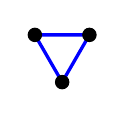
\begin{tikzpicture}[scale=0.5]
    \draw \foreach \x in {0,1,2}{(270+\x*360/3:0.8) coordinate(x\x)};
    \draw[edge_color2] (x0)--(x1)--(x2)--(x0);
    \draw (x0) node[unlabeled_vertex]{};
    \draw (x1) node[unlabeled_vertex]{};
    \draw (x2) node[unlabeled_vertex]{};
  \end{tikzpicture}}
}
\newcommand{\kthree}{\flagone}

\newcommand{\flagtwo}{ % this is the unlabeled edge
  \vc{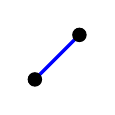
\begin{tikzpicture}[scale=0.5]
    \draw (225:0.8) coordinate(x0);
    \draw (45:0.8) coordinate(x1);
    \draw[edge_color2] (x0)--(x1);
    \draw (x0) node[unlabeled_vertex]{};
    \draw (x1) node[unlabeled_vertex]{};
  \end{tikzpicture}}
}
\newcommand{\edge}{\flagtwo}

\newcommand{\flagthree}{ % this represents the edges among non-neighbors of a vertex
  \vc{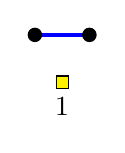
\begin{tikzpicture}[scale=0.5]
    \draw \foreach \x in {0,1,2}{(270+\x*360/3:0.8) coordinate(x\x)};
    \draw[edge_color2] (x1)--(x2);
    \draw (x0) node[labeled_vertex,label=below:$1$]{};
    \draw (x1) node[unlabeled_vertex]{};
    \draw (x2) node[unlabeled_vertex]{};
  \end{tikzpicture}}
}

\newcommand{\flagfour}{
  \vc{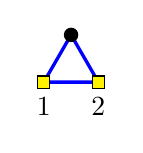
\begin{tikzpicture}[scale=0.5]
    \draw \foreach \x in {0,1,2}{(210+\x*360/3:0.8) coordinate(x\x)};
    \draw[edge_color2] (x0)--(x1)--(x2)--(x0);
    \draw (x0) node[labeled_vertex,label=below:$1$]{};
    \draw (x1) node[labeled_vertex,label=below:$2$]{};
    \draw (x2) node[unlabeled_vertex]{};
  \end{tikzpicture}}
}
\newcommand{\kthreeLabeledEdge}{\flagfour}

\newcommand{\flagfive}{ % this is the labeled edge
  \vc{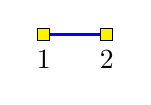
\begin{tikzpicture}[scale=0.5]
    \draw (180:0.8) coordinate(x0);
    \draw (360:0.8) coordinate(x1);
    \draw[edge_color2] (x0)--(x1);
    \draw (x0) node[labeled_vertex,label=below:$1$]{};
    \draw (x1) node[labeled_vertex,label=below:$2$]{};
  \end{tikzpicture}}
}
\newcommand{\labeledEdge}{\flagfive}

\newcommand{\flagsix}{ % this is the labeled non-edge
  \vc{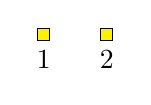
\begin{tikzpicture}[scale=0.5]
    \draw (180:0.8) coordinate(x0);
    \draw (360:0.8) coordinate(x1);
    \draw (x0) node[labeled_vertex,label=below:$1$]{};
    \draw (x1) node[labeled_vertex,label=below:$2$]{};
  \end{tikzpicture}}
}
\newcommand{\labeledNonEdge}{\flagsix}

\newcommand{\flagseven}{
  \vc{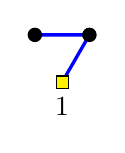
\begin{tikzpicture}[scale=0.5]
    \draw \foreach \x in {0,1,2}{(270+\x*360/3:0.8) coordinate(x\x)};
    \draw[edge_color2] (x0)--(x1)--(x2);
    \draw (x0) node[labeled_vertex,label=below:$1$]{};
    \draw (x1) node[unlabeled_vertex]{};
    \draw (x2) node[unlabeled_vertex]{};
  \end{tikzpicture}}
}

\newcommand{\flageight}{ % this is the labeled edge with an extra vertex joined to 1
  \vc{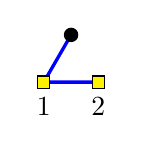
\begin{tikzpicture}[scale=0.5]
    \draw \foreach \x in {0,1,2}{(210+\x*360/3:0.8) coordinate(x\x)};
    \draw[edge_color2] (x2)--(x0)--(x1);
    \draw (x0) node[labeled_vertex,label=below:$1$]{};
    \draw (x1) node[labeled_vertex,label=below:$2$]{};
    \draw (x2) node[unlabeled_vertex]{};
  \end{tikzpicture}}
}

\newcommand{\flagnine}{ % this is the labeled edge with an extra vertex joined to 2
  \vc{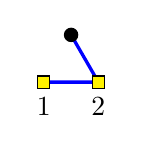
\begin{tikzpicture}[scale=0.5]
    \draw \foreach \x in {0,1,2}{(210+\x*360/3:0.8) coordinate(x\x)};
    \draw[edge_color2] (x0)--(x1)--(x2);
    \draw (x0) node[labeled_vertex,label=below:$1$]{};
    \draw (x1) node[labeled_vertex,label=below:$2$]{};
    \draw (x2) node[unlabeled_vertex]{};
  \end{tikzpicture}}
}

\newcommand{\flagten}{
  \vc{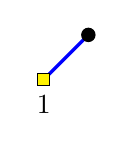
\begin{tikzpicture}[scale=0.5]
    \draw (225:0.8) coordinate(x0);
    \draw (45:0.8) coordinate(x1);
    \draw[edge_color2] (x0)--(x1);
    \draw (x0) node[labeled_vertex,label=below:$1$]{};
    \draw (x1) node[unlabeled_vertex]{};
  \end{tikzpicture}}
}
\newcommand{\edgeWithOneLabel}{\flagten}

\newcommand{\flageleven}{
  \vc{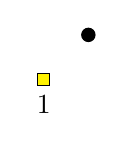
\begin{tikzpicture}[scale=0.5]
    \draw (225:0.8) coordinate(x0);
    \draw (45:0.8) coordinate(x1);
    \draw (x0) node[labeled_vertex,label=below:$1$]{};
    \draw (x1) node[unlabeled_vertex]{};
  \end{tikzpicture}}
}
\newcommand{\nonEdgeWithOneLabel}{\flageleven}

\newcommand{\flagtwelve}{
  \vc{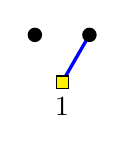
\begin{tikzpicture}[scale=0.5]
    \draw \foreach \x in {0,1,2}{(270+\x*360/3:0.8) coordinate(x\x)};
    \draw[edge_color2] (x0)--(x1);
    \draw (x0) node[labeled_vertex,label=below:$1$]{};
    \draw (x1) node[unlabeled_vertex]{};
    \draw (x2) node[unlabeled_vertex]{};
  \end{tikzpicture}}
}

Nesse capítulo, introduzimos alguns aspectos do poderoso método de álgebras de flag, introduzido por Razborov em 2007~\cite{razborov2007flag}.
O método tem sido usado de forma diversa para obter resultados acerca de problemas em combinatória extremal, particularmente pela sua capacidade expressiva de representar densidades e homomorfismos de estruturas combinatórias variadas (grafos, grafos orientados, permutações...)
Para uma visão histórica do uso das álgebras de flag e resultados importantes alcançados ainda nos primeiros anos após a introdução do método, recomendamos~\cite{razborov2013survey}.

Nesse capítulo, introduzimos a teoria de álgebras de flag aplicada a grafos simples e densidades de subgrafos.
A estrutura é fortemente baseada na exposição de~\cite{grzesik2014thesis} e também em~\cite{marcel2016flag}.
Deixamos muitos dos detalhes técnicos das definições de lado em um primeiro momento, focando em uma abordagem prática que motive a utilização das álgebras de flag para problemas extremais em grafos livres de triângulos.

%!TeX root=../tese.tex
\section{Conceitos iniciais}

\subsection{Densidades}\label{sub:densidades}
Sejam $F$ e $G$ grafos quaisquer.
Definimos a \emph{densidade de $F$ em $G$} (denotada $d(F,G)$) como o número de subgrafos induzidos de $G$ com $|F|$ vértices que são isomorfos a $F$.
Analogamente, $d(F,G)$ é a probabilidade que um conjunto de $|F|$ vértices de $G$, escolhido uniformemente ao acaso, induza um subgrafo isomorfo a $F$.

Fixe um grafos $F$ e $G$ com $|F| \leq |G|$.
Para calcular $d(F,G)$, podemos escolher um inteiro $l$ com $|F| \leq l \leq |G|$ e escrever
\begin{equation}\label{eq:chain-rule}
  d(F,G) = \sum_{|V(H)|=l} d(F,H)d(H,G).
\end{equation}
A igualdade é válida porque amostrar um subconjunto $S \subseteq \binom{V(G)}{l}$ uniformemente ao acaso e depois amostrar um subconjunto $T \subseteq \binom{S}{|F|}$ segue a distribuição uniforme em $\binom{V(G)}{|F|}$.

Agora, denote por $\calf_l^\emptyflag$ a família dos grafos livres de triângulos com $l$ vértices (a menos de isomorfismo).
Para a configuração geral de álgebras de flag, a família ``proibida'' pode ser qualquer conjunto finito de grafos, que no nosso caso é simplesmente $\{K_3\}$.
Se $G$ é um grafo livre de triângulos, então por (\ref{eq:chain-rule}) vale que
\begin{equation}\label{eq:chain-rule-2}
  d(F,G) = \sum_{H \in \calf_l^\emptyflag} d(F,H)d(H,G).
\end{equation}
Essa expressão é comumente referida como uma \emph{regra da cadeia} no contexto de álgebras de flag.

Muitos problemas típicos em Teoria Extremal dos Grafos, como o próprio Teorema de Mantel, são problemas de minimização de uma expressão do tipo $d(F,G)$, e frequentemente desejamos utilizar~(\ref{eq:chain-rule-2}) para simplificar os cálculos de densidade.
Por exemplo, usando $\sum_{H \in \calf_l^\emptyflag} d(H,G)= 1$ temos $d(F,G) \leq \max_{H \in \calf_l^\emptyflag} d(F,H)$.
Essa cota é um resultado ``finito'', pois enquanto $G$ é um grafo em geral muito maior que $F$, o parâmetro $l$ é algo que podemos tentar controlar para obter resultados mais refinados.

Contudo, essa cota em geral é bastante fraca, e um grande desafio é de gerar desigualdades lineares entre densidades que sejam mais sofisticadas que a regra da cadeia.
Mais especificamente, seria interessante ter desigualdades da forma
\begin{equation}\label{eq:cH-inequality}
  \sum_{H \in \calf_l^\emptyflag} c_H d(H,G) \geq 0,
\end{equation}
onde os $c_H$'s' são constantes reais, potencialmente negativas, que possam ser usadas para balancear as densidades de um e outro subgrafo de $G$.
Logo, poderíamos obter de (\ref{eq:chain-rule-2}) a desigualdade
\[ d(F,G) \leq \sum_{H \in \calf_l^\emptyflag} (c_H+d(F,H))d(H,G) \leq \max_{H \in \calf_l^\emptyflag} \left(c_H+d(F,H)\right). \]
Novamente, esse tipo de desigualdade permitirá cotar superiormente o valor de $d(F,G)$ para grafos ``grandes'' $G$ usando apenas informações ``finitas'', vindas de $F$, de $l$ e da desigualdade na forma de (\ref{eq:cH-inequality}).

Na verdade, o \emph{método semidefinido} permitirá obter desigualdades na forma
\begin{equation}\label{eq:cH-inequality-o(1)}
  \sum_{H \in \calf_l^\emptyflag} c_H d(H,G) + o(1) \geq 0,
\end{equation}
onde o termo $o(1)$ vai para zero quando $|G|$ cresce, e portanto a cota superior obtida para $d(F,G)$ será
\begin{equation}\label{eq:max-bound}
  d(F,G) \leq \max_{H \in \calf_l^\emptyflag} \left(c_H + d(F,H)\right) + o(1).
\end{equation}
Em geral, esse tipo de resultado é suficiente quando a compreensão assintótica é suficiente.
Veremos no caso do Teorema~\ref{thm:mantel} e posteriormente no caso da Conjectura~\ref{conj:make-bipartite} que argumentos com blow-ups podem ser usadas para transferir os resultados assintóticos para grafos de qualquer tamanho finito.
Ou seja, o termo $o(1)$ em (\ref{eq:cH-inequality-o(1)}) poderá ser controlado para as aplicações visadas nesse trabalho.

\subsection{O Teorema de Mantel}

Nessa seção, iremos provar o Teorema~\ref{thm:mantel} usando técnicas de álgebras flag que são simples descrever e que serão generalizadas no que se segue da exposição do método geral.
Iremos usar representações visuais para grafos como usual, de forma que $\edge$ é um grafo isomorfo a $K_2$, $\unlabeledCherry$ é um grafo isomorfo a $(\{a,b,c\},\{ab,ac\})$ e assim por diante.
A motivação para isso, além de facilitar a leitura, é de deixar claro constantemente quais grafos são ``pequenos'' e podem ser vistos como parâmetros ou variáveis do método, enquanto quando escrevermos $G$ para representar um grafo como em $d\left(\unlabeledCherry,G\right)$, tipicamente estamos pensando em $G$ como um grafo com $n$ vértices e no comportamento assintótico dessa densidade quando $n \to +\infty$.

O Teorema de Mantel pode ser reescrito na forma
\[ d\left(\edge,G\right) \leq \frac{\frac{n^2}{4}}{\binom{n}{2}} = \frac12+o(1),\] onde $G$ é um grafo livre de triângulos com $n$ vértices, e o termo de erro $o(1)$ que vai para zero quando $n \to +\infty$.


Usando $l=3$ em~(\ref{eq:chain-rule-2}), temos
\[ d\left(\edge,G\right) = d\left(\edge,\threePoints\right)d\left(\threePoints,G\right) + d\left(\edge,\unlabeledCherryComplement\right)d\left(\unlabeledCherryComplement,G\right) + d\left(\edge,\unlabeledCherry\right)d\left(\unlabeledCherry,G\right), \]
ou simplesmente
\begin{equation}\label{eq:mantel-basic}
  d\left(\edge,G\right) = \frac13d\left(\unlabeledCherryComplement,G\right)+\frac23d\left(\unlabeledCherry,G\right).
\end{equation}

Com isso, vemos que $d\left(\edge,G\right) \leq 2/3$.
Mas isso é bem mais fraco que o Teorema de Mantel, então vamos buscar uma desigualdade na forma de~(\ref{eq:cH-inequality-o(1)}) que nos permita concluir $d\left(\edge,G\right) \leq 1/2+o(1)$.

A desigualdade em questão será
\begin{equation}\label{eq:mantel-carteada}
  \frac12d\left(\threePoints,G\right)-\frac16d\left(\unlabeledCherryComplement,G\right)-\frac16d\left(\unlabeledCherry,G\right)+o(1) \geq 0.
\end{equation}
Assumindo~(\ref{eq:mantel-carteada}) e somando com~(\ref{eq:mantel-basic}), temos \[ d\left(\edge,G\right) \leq \frac12d\left(\threePoints,G\right)+\frac16d\left(\unlabeledCherryComplement,G\right)+\frac12d\left(\unlabeledCherry,G\right)+o(1) \leq \frac12+o(1), \]
como desejado.
Então nos resta descobrir como gerar a desigualdade ``mágica'' de~(\ref{eq:mantel-carteada}).

Fixe um vértice ``especial'' $v \in V(G)$ (que representaremos como $\aSinglePoint$).
Definimos densidades em $G^{\aSinglePoint}$ com um vértice especial da mesma forma que quando $G$ não tinha vértices especiais, mas agora calculando a densidade de subestruturas que também tenham um vértice especial.
Por exemplo, $d\left(\edgeWithOneLabel,G^{\aSinglePoint}\right)$ é a probabilidade de que um vértice $u \in V(G)\setminus\{v\}$, escolhido uniformemente ao acaso, seja vizinho de $G$.

Observe que
\begin{equation}\label{eq:quadratic-ineq}
  \left(d\left(\edgeWithOneLabel,G^{\aSinglePoint}\right)-d\left(\nonEdgeWithOneLabel,G^{\aSinglePoint}\right)\right)^2 \geq 0,
\end{equation}
e portanto
\begin{equation}\label{eq:flag-squared-expanded}
  d\left(\edgeWithOneLabel,G^{\aSinglePoint}\right)^2 - 2d\left(\edgeWithOneLabel,G^{\aSinglePoint}\right)d\left(\nonEdgeWithOneLabel,G^{\aSinglePoint}\right) + d\left(\nonEdgeWithOneLabel,G^{\aSinglePoint}\right)^2 \geq 0.
\end{equation}
O produto $d\left(\edgeWithOneLabel,G^{\aSinglePoint}\right)^2$ é a probabilidade que dois vértices escolhidos aleatoriamente ao acaso (com reposição) em $V(G) \setminus \{v\}$ sejam ambos vizinhos de $G$.
A probabilidade que esses dois vértices sejam iguais é $o(1)$ quando $n \to +\infty$, e se eles são distintos, então os dois (junto com $v$) induzem um subgrafo isomorfo a $\labeledCherry$ (pois $G$ é livre de triângulos).
Ou seja, \[d\left(\edgeWithOneLabel,G^{\aSinglePoint}\right)^2 = d\left(\labeledCherry,G^{\aSinglePoint}\right)+o(1).\]

De forma análoga, é possível provar
\begin{align}
  d\left(\edgeWithOneLabel,G^{\aSinglePoint}\right) d\left(\nonEdgeWithOneLabel,G^{\aSinglePoint}\right) &= \frac12d\left(\asymmetricLabeledCherry,G^{\aSinglePoint}\right)+\frac12d\left(\asymmetricLabeledCherryComplement,G^{\aSinglePoint}\right)+o(1), \label{eq:linearize-1} \\
  d\left(\nonEdgeWithOneLabel,G^{\aSinglePoint}\right)^2 &= d\left(\labeledCherryComplement,G^{\aSinglePoint}\right)+d\left(\threePointsWithOneLabel,G^{\aSinglePoint}\right)+o(1). \label{eq:linearize-2}
\end{align}

Substituindo (\ref{eq:linearize-1}) e (\ref{eq:linearize-2}) em
(\ref{eq:flag-squared-expanded}), obtemos
\begin{equation}\label{eq:ineq-in-Gsigma}
   d\left(\labeledCherry,G^{\aSinglePoint}\right)-d\left(\asymmetricLabeledCherry,G^{\aSinglePoint}\right)-d\left(\asymmetricLabeledCherryComplement,G^{\aSinglePoint}\right)+d\left(\labeledCherryComplement,G^{\aSinglePoint}\right)+d\left(\threePointsWithOneLabel,G^{\aSinglePoint}\right) + o(1) \geq 0.
\end{equation}
Obtivemos assim uma igualdade que se assemelha à igualdade (\ref{eq:mantel-carteada}), mas com densidades de conjuntos de $3$ vértices contendo um vértice especial $v$ de $G^{\aSinglePoint}$ em vez de densidades em $G$ para subconjuntos de tamanho $3$ escolhidos ao acaso e sem vértices especiais.

Para obter a relação desejada, iremos escolher $v$ uniformemente ao acaso!
Isso também pode ser pensado de forma determinística como a média de~(\ref{eq:ineq-in-Gsigma}) por todas as escolhas possíveis de $v \in V(G)$.

Escolhendo $v$ aleatoriamente, temos que
\[ \bbe\left[d\left(\labeledCherry,G^{\aSinglePoint}\right)\right] = \frac13d\left(\unlabeledCherry,G\right), \]
pois para cada subgrafo induzido de $G$ que é isomorfo a $\unlabeledCherry$ existe apenas uma dentre as três escolhas possíveis para o vértice especial $v$ tal que o grafo ``rotulado'' resultante é isomorfo a $\labeledCherry$.
De forma similar, temos

\[\bbe\left[d\left(\asymmetricLabeledCherry,G^{\aSinglePoint}\right)\right] = \frac23d\left(\unlabeledCherry,G\right), \qquad \bbe\left[d\left(\asymmetricLabeledCherryComplement,G^{\aSinglePoint}\right)\right] = \frac23d\left(\unlabeledCherryComplement,G\right),\]
\[\bbe\left[d\left(\labeledCherryComplement,G^{\aSinglePoint}\right)\right] = \frac13d\left(\unlabeledCherryComplement,G\right), \qquad \bbe\left[d\left(\threePointsWithOneLabel,G^{\aSinglePoint}\right)\right] = d\left(\threePoints,G\right).\]

Portanto, segue de (\ref{eq:ineq-in-Gsigma}) que
\[ \frac13d\left(\unlabeledCherry,G\right)-\frac23d\left(\unlabeledCherry,G\right)-\frac23d\left(\unlabeledCherryComplement,G\right)+\frac13d\left(\unlabeledCherryComplement,G\right)+d\left(\threePoints,G\right)+o(1) \geq 0, \]
que é o mesmo que
\[ d\left(\threePoints,G\right)-\frac13d\left(\unlabeledCherryComplement,G\right)-\frac13d\left(\unlabeledCherry,G\right)+o(1) \geq 0, \]
que é um múltiplo de (\ref{eq:mantel-carteada}).
Assim, provamos que se $G$ é um grafo livre de triângulos, então $d\left(\edge,G\right) \leq 1/2+o(1)$.

Para provar a versão original do Teorema de Mantel (ou seja, que $e(G) \leq n^2/4$ em vez de $e(G) \leq n^2/4+o(n^2)$), tome um grafo livre de triângulos $G$ qualquer e considere blow-up balanceado $G_N$ de $G$ em que cada vértice de $G$ é substituído por um conjunto independente de tamanho $N$.
Então, pela versão assintótica do Teorema de Mantel que provamos, $e(G_N) \leq \frac12\binom{N|G|}{2} + o(1) \leq \frac{N^2|G|^2}{4}+o(N^2)$.
Além disso, $e(G) = N^2e(G)$, portanto $e(G) \leq \frac{|G|^2}{4}+\frac{o(N^2)}{N^2}$.
Fazendo $N \to \infty$, obtemos $e(G) \leq \frac{|G|^2}{4}$, pois $e(G)$ é inteiro.
Esse argumento conclui a prova do Teorema de Mantel.

A estratégia apresentada no esboço acima reflete bem a estratégia geral que utilizaremos quando formos provar algum resultado mais sofisticado com álgebras de flag:
\begin{enumerate}
  \item Começamos fixando um subgrafo especial $\sigma$ (no caso de Mantel, $\sigma = \aSinglePoint$ tem apenas um vértice) para uma desigualdade quadrática (\ref{eq:quadratic-ineq}) envolvendo as densidades relativas a uma cópia fixa de $\sigma$ em $G$;
  \item Multiplicamos tais densidades relativas a $\sigma$ adicionando termos de erro para obter desigualdades lineares com as densidades relativas a $\sigma$ (\ref{eq:linearize-1});
  \item Escolhemos aleatoriamente um subgrafo induzido de $G$ isomórfico a $\sigma$ para associar as densidades de subgrafos com $\sigma$ fixado a densidades de subgrafos sem essa restrição.
\end{enumerate}

A princípio, todos os passos acima podem ser automatizados, exceto a obtenção da desigualdade quadrática inicial.
Essa desigualdade deve satisfazer a hipótese de ser não negativa para toda escolha de densidade envolvida.


Uma forma de obter isso é escolher uma desigualdade da forma $v^\top A v \geq 0$, onde $v$ é um vetor com todas as densidades de certos subgrafos bem escolhidos e $A$ é uma matriz positiva semidefinida.
Por exemplo, podemos reescrever (\ref{eq:flag-squared-expanded}) como
\[
  \begin{bmatrix}
  d\left(\edgeWithOneLabel,G^{\aSinglePoint}\right) & d\left(\nonEdgeWithOneLabel,G^{\aSinglePoint}\right)
  \end{bmatrix}
  \begin{bmatrix}
    1 & -1 \\
    -1 & 1
  \end{bmatrix}
  \begin{bmatrix}
  d\left(\edgeWithOneLabel,G^{\aSinglePoint}\right) \\
  d\left(\nonEdgeWithOneLabel,G^{\aSinglePoint}\right)
  \end{bmatrix}
  \geq 0.
\]

De fato, poderíamos ter começado com uma matriz positiva semidefinida genérica $A=\begin{bmatrix} a_{11} & a_{12} \\ a_{12} & a_{22} \end{bmatrix}$.
Encontrando os coeficientes de~(\ref{eq:cH-inequality-o(1)}) e cotando em~(\ref{eq:max-bound}), poderíamos provar então que $d(\edge,G) \leq d^*+o(1)$, onde $d^*$ é o valor ótimo do programa semidefinido
\begin{alignat*}{1}
  \text{Minimizar} \quad
  & \max\left\{\frac23+\frac13a_{11}+\frac23a_{12}, \frac13 + \frac23a_{12}+\frac13a_{22},a_{22}\right\}\\
  \text{sujeito a}
  \quad & \begin{bmatrix}
    a_{11} & a_{12} \\
    a_{12} & a_{22}
  \end{bmatrix} \in \bbs_+^2.
\end{alignat*}

\subsection{Tipos e o método semidefinido geral}

Seja $\calf$ uma família de grafos ``proibidos''.
Um \emph{tipo} $\sigma$ é um grafo $\calf$-livre associado a uma bijeção $\theta \colon [s] \to V(\sigma)$ para algum $s \geq 0$.
Frequentemente iremos omitir a bijeção quando essa for clara do contexto.
Um \emph{$\sigma$-flag} é um grafo $\calf$-livre $F$ que contém como subgrafo induzido uma cópia de $\sigma$ rotulada por $\theta$.
Em outras palavras, um tipo é um grafo (pequeno) com todos os seus vértices rotulados/especiais, enquanto um flag é um grafo parcialmente rotulado de acordo com um tipo.

Dado um grafo $G$ e um tipo $\sigma$ de tamanho $s$, vamos fixar inteiros $l \geq s$ e $m \leq (l+s)/2$.
Seja $\calf_m^\sigma$ o conjunto de todos os $\sigma$-flags de tamanho $m$, a menos de isomorfismo (no caso de flags, o isomorfismo deve preservar os rótulos da bijeção $\theta$ na parte rotulada dos grafos).
Seja também $\Theta$ o conjunto de todos os homorfismos injetivos de $[s]$ para $V(G)$.
Dado $F \in \calf_m^\sigma$ e $\theta \in \Theta$, definimos a \emph{densidade induzida} $d(F,G;\theta)$ como a probabilidade de um conjunto $V' \subseteq V(G)$ de tamanho $m$ que contém $\sigma$, escolhido uniformemente ao acaso, induza um $\sigma$-flag isomórifico a $F$.
Observe que para $s=0$ (isto é, quando o grafo não possui vértices rotulados), então $d(F,G;\theta)=d(F,G)$ é a definição usual de densidade induzida.

Se $F_a,F_b \in \calf_m^\sigma$ e $\theta \in \Theta$, definimos $d(F_a,F_b,G;\theta)$ como a probabilidade de, ao escolhermos dois conjuntos $V_a,V_b \subseteq V(G)$ com $V_a \cap V_b = \mathrm{im}(\theta)$, uniformemente ao acaso, então os $\sigma$-flags induzidos por $V_a$ e $V_b$ são isomórficos a $F_a$ e $F_b$ respectivamente.
Essa definição é importante para lidar com produtos de densidades, como diz o próximo teorema:
\begin{theorem}[\cite{razborov2007flag}]\label{thm:multiplying-densities}
  Para $F_a,F_b \in \calf_m^\sigma$ e $\theta \in \Theta$, vale
  \[ d(F_a,G;\theta)d(F_b,G;\theta) = d(F_a,F_b,G;\theta) + o(1), \]
  onde o termo $o(1)$ vai para zero quando $|G|$ vai para infinito.
\end{theorem}

Seja $\calf_m^\sigma=\{F_1,F_2,\dots,F_\ell\}$ e sejam $v \in \bbr^{\ell}$ um vetor e uma matriz positiva semidefinida $Q \in \mathcal{S}^\ell_+$.
Então de $v^\top Q v \geq 0$, podemos escrever
%\[ \sum_{F_a,F_b \in \calf_m^\sigma} Q_{ab} v_a v_b \geq 0. \]
\[ \sum_{i,j=1}^{\ell} Q_{ij}v_iv_j \geq 0. \]
Fazendo $v_i = d(F_i,G;\theta)$ e usando o Teorema~\ref{thm:multiplying-densities}, obtemos
\begin{equation}\label{eq:1}
  %\sum_{F_i,F_j \in \calf_m^\sigma} Q_{ij} d(F_i,F_j,G;\theta) + o(1) \geq 0.
  \sum_{i,j=1}^{\ell}Q_{ij}d(F_i,F_j,G;\theta) + o(1) \geq 0.
\end{equation}

Agora, seja $H \in \calf_l^\emptyset$ um flag sem vértices rotulados e seja $\Theta_H$ o conjunto de homorfismos injetivos de $[s]$ para $V(H)$.
Da mesma forma que em (\ref{eq:chain-rule-2}), é fácil ver que
\begin{equation}\label{eq:2}
  \bbe_{\theta \in \Theta}\left[d(F_i,F_j,G;\theta)\right] = \sum_{H \in \calf_l^\emptyflag} \bbe_{\theta \in \Theta_H}\left[d(F_i,F_j,H;\theta)\right]d(H,G).
\end{equation}

De (\ref{eq:1}) e (\ref{eq:2}), temos então
\[ \sum_{H \in \calf_l^{\emptyflag}} \sum_{i,j=1}^{\ell} Q_{ij} \bbe_{\theta \in \Theta_H} \left[d(F_i,F_j,H;\theta)\right] d(H,G) + o(1) \geq 0. \]
Definindo $c_H(\sigma,m,Q) \coloneqq \sum_{i,j=1}^{\ell} Q_{ij} \bbe_{\theta \in \Theta_H} \left[d(F_i,F_j,H;\theta)\right]$, a desigualdade obtida é exatamente da forma
\begin{equation}\label{eq:general-density-ineq}
  \sum_{H \in \calf_l^\emptyflag} c_H(\sigma,m,Q)d(H,G) + o(1) \geq 0.
\end{equation}

Combinando (\ref{eq:chain-rule-2}) e (\ref{eq:general-density-ineq}) para montar um programa semidefinido adequado, é possível obter cotas para os chamados ``problemas do tipo Turán'' ao variar os hiperparâmetros $m,l,\sigma$ do modelo e utilizar a cota de (\ref{eq:max-bound}).
Também é possível combinar escolhas de hiperparâmetros $c_H(\sigma_i,m_i,Q_i)$ para obter cotas mais refinadas (ver~\cite{grzesik2012pentagon}).
Essas ideias renderam vários resultados importantes desde a introdução do método de álgebras de flag, em particular com o prolífico software \texttt{flagmatic} (\href{https://lidicky.name/flagmatic/}), que implementa a abordagem descrita nessa seção.

\subsection{A álgebra}

Agora que introduzimos os conceitos e objetivos gerais quando estamos resolvendo um problema usando álgebras de flag, vamos formalizar alguns dos conceitos que apresentamos para simplificar as aplicações posteriores.
Como visto, o objetivo geral do método aplicado a problemas de densidade e homomorfismos é obter desigualdades não triviais da forma
\begin{equation}\label{eq:3}
  \sum_{F_i \in \calf_l^\emptyflag} a_i d(F_i,G) + o(1) \geq 0,
\end{equation}
onde $l$ é fixo e $G \in \calf^\emptyflag$ é um grafo (não rotulado) arbitrário.
Para isso, vimos que é interessante considerar desigualdades na forma $\sum_{F_i \in \calf_l^\sigma} a_i d(F_i,G) + o(1) \geq 0$, onde $G \in \calf^\sigma$ é um grafo ``grande'' e aplicar um operador linear (associado a uma distribuição de probabilidade) que gere uma desigualdade da forma de (\ref{eq:3}).

Como pensamos em $G$ como grande e arbitrário, podemos ver as somas $\sum_{F_i \in \calf_l^\emptyflag} a_i d(F_i,G)$ como ações de $\calf^\sigma$ sobre $\bbr\calf^\sigma$.
Ou seja, vamos considerar as somas formais de $\sigma$-flags e deixar um grafo $G$ agir sobre elas através de $\sum_{i \in I} a_iF_i \mapsto \sum_{i \in I} a_id(F_i,G_i)$.
Note que, de~(\ref{eq:chain-rule-2}), todo elemento da forma
\begin{equation}\label{eq:guys-in-kernel}
  \tilde F-\sum_{F \in \calf_l^\sigma} d(\tilde F, F)F
\end{equation}
é levado a $0$ por qualquer por $G$.
Defina o espaço quociente $\cala^\sigma \coloneqq \bbr\calf^\sigma/\calk^\sigma$, onde $\calk^\sigma$ é o subespaço gerado pelos elementos da forma~(\ref{eq:guys-in-kernel}).

Finalmente, é importante definir uma noção adequada de multiplicação nesse espaço vetorial para manipular a multiplicação de densidades.
Assim, também transformaremos $\cala^\sigma$ numa álgebra.
Para $F_1 \in \calf_{l_1}^\sigma$ e $F_2 \in \calf_{l_2}^\sigma$ e $l \geq l_1+l_2-|\sigma|$, definimos
\[ F_1 \cdot F_2 = \sum_{F \in \calf_l^\sigma} d(F_1,F_2,F)F, \]
e definimos a multiplicação sobre $\cala^\sigma$ expandindo essa definição bilinearmente.
É possível provar (ver~\cite{razborov2007flag}) que essa operação de multiplicação está bem definida em $\cala^\sigma$, ou seja, que não depende da escolha de $l$.
Defina o mapa
\[ \phi_G \colon \sum a_iF_i \in \cala^\sigma \mapsto \sum a_id(F_i,G) \in \bbr. \]
Pelo Teorema~\ref{thm:multiplying-densities}, $\phi_G$ pode ser visto como um ``homomorfismo aproximado'' de $\cala^\sigma$ para $\bbr$.

Por clareza, apresentamos alguns exemplos de igualdades em $\cala^{\emptyflag}$ e em $\cala^{\aSinglePoint}$:
\begin{align*}
  \edge &= \frac13\unlabeledCherryComplement + \frac23\unlabeledCherry + \kThree, \\
  \edgeWithOneLabel \cdot \edgeWithOneLabel &= \labeledCherry + \kThreeWithOneLabel, \\
  \edgeWithOneLabel \cdot \nonEdgeWithOneLabel &= \frac12 \asymmetricLabeledCherryComplement + \frac12 \asymmetricLabeledCherry.  
\end{align*}

Muitas vezes, quando estamos querendo provar algum resultado de densidade, começamos com desigualdades de densidades com vértices especiais rotulados de acordo com um tipo $\sigma$.
Para transferir esse resultado para grafos não rotulados (i.e., $\emptyflag$-flags), escolhemos aleatoriamente onde alocar $\sigma$ em $G$.
Em álgebras de flag, esse formalismo será realizado por operadores lineares
\[ \average{\cdot} \colon \cala^\sigma \to \cala^\emptyflag \]
que representam essa ``média''.

Para $F \in \calf^\sigma$, definimos $\average{F} \coloneqq q(F)\downward F$, onde $\downward F \in \calf^\emptyflag$ é uma cópia de $F$ em que os rótulos especiais são esquecidos, e $q(F)$ é a probabilidade que a imagem de um homorfismo injetivo $\theta \colon [|\sigma|] \to V(\downward F)$ escolhido uniformemente ao acaso defina um flag isomórfico a $F$.
Em seguida, estendemos $\average{\cdots}$ linearmente para $\cala^\sigma$.
Por exemplo, temos
\[
  \average{\edgeWithOneLabel} = \edge, \qquad
  \average{2\labeledCherry+\asymmetricLabeledCherry} = \frac43\unlabeledCherry, \qquad
  \average{\cherryWithLabeledEdge} = \frac13 \unlabeledCherry.
\]
Note que os $\left(\labeledEdge\right)$-flags $\cherryWithLabeledEdge$ e $\anotherCherryWithLabeledEdge$ não são isomórficos.
Como esse tipo tem mais de um vértice, é importante rotulá-los.
Ao contrário, no tipo de tamanho $1$ o rótulo não é relevante.

Finalmente, iremos lidar com a noção de ``homomorfismos aproximados'' de $\cala^\sigma$ a $\bbr$ e como recuperar de toda a linguagem algébrica introduzida a informação sobre densidades em grafos para o problema original.
Para cada $\sigma$-flag $G$, podemos associar um vetor (de dimensão infinita) $\left(d(F,G)\right)_{F \in \calf^\sigma} \in [0,1]^{\calf^\sigma}$.
Se $(G_k)_{k \geq 0}$ é uma sequência de $\sigma$-flags tal que tal que $d(F,G_k)$ converge para todo $F \in \calf^\sigma$, então dizemos que $(G_k)_{k \geq 0}$ é \emph{convergente}.
Pela compacidade de $[0,1]$ e o Teorema de Tychonoff, o espaço $[0,1]^{\calf^\sigma}$ com a topologia produto é compacto.
Logo, toda sequência infinita $(G_k)_{k \geq 0}$ de $\sigma$-flags possui uma subsequência infinita que é convergente.

Para cada sequência convergente $(G_k)_{k \geq 0}$ em $[0,1]^{\calf^\sigma}$, existe um homomorfismo (entre espaços vetoriais)
\[ \phi \colon F \in \calf^\sigma \mapsto \lim_{k \to +\infty} d(F,G_k) \in \bbr\] que pode ser estendido para um homomorfismo (entre álgebras) $\phi \colon \cala^\sigma \to \bbr$.
Esses homomorfismos serão chamados de \emph{homomorfismos funcionais}.
Dessa forma, se vale uma desigualdade $\sum a_iF_i \geq 0$ em $\cala^\sigma$, então também vale $\phi\left(\sum a_iF_i\right) \geq 0$ para todo homomorfismo funcional $\phi$, e logo $\sum a_id(F_i,G_k) + o(1) \geq 0$ para toda sequência convergente $(G_k)_{k \geq 0}$, onde o termo $o(1)$ vai para zero quando $|G_k|$ vai para infinito.
Escolher $(G_k)_{k \geq 0}$ como uma sequência de blow-ups balanceados de um grafo base será suficiente para as aplicações desse trabalho.

Vamos mostrar mais uma vez o Teorema de Mantel usando a expressiva da álgebra que acabamos de desenvolver.
Começamos com \[\left(\edgeWithOneLabel - \nonEdgeWithOneLabel\right)^2 \geq 0.\]
Daí, temos \[ \edgeWithOneLabel\cdot\edgeWithOneLabel-2\ \edgeWithOneLabel\cdot\nonEdgeWithOneLabel+\nonEdgeWithOneLabel\cdot\nonEdgeWithOneLabel \geq 0, \]
e multiplicando obtemos \[ \labeledCherry - \asymmetricLabeledCherry - \asymmetricLabeledCherryComplement + \labeledCherryComplement + \threePointsWithOneLabel \geq 0. \]
Aplicando $\average{\cdot}$, segue que \[ \frac13\unlabeledCherry -\frac23\unlabeledCherry - \frac23\unlabeledCherryComplement + \frac13\unlabeledCherryComplement + \threePoints \geq 0 \implies \threePoints - \frac13 \unlabeledCherryComplement - \frac13\unlabeledCherry \geq 0. \]
Dividindo por $2$ e somando a igualdade \[ \edge = \frac13\unlabeledCherryComplement + \frac23\unlabeledCherry, \]
obtemos \[ \edge \leq \frac12\threePoints + \frac16\unlabeledCherryComplement + \frac12\unlabeledCherry \leq \frac12. \]

Logo, toda sequência infinita de grafos livres de triângulos $(G_k)_{k \geq 0}$ possui uma subsequência $(G_{i_k})_{k \geq 0}$com $d\left(\edge,G_{i_k}\right) \leq 1/2 + o(1)$.
Tome $G_1$ qualquer e para cada $N \geq 2$ defina $G_N$ como um blow-up completo balanceado de $G_0$ em que cada vértice de $G_0$ é substituído por um conjunto independente de tamanho $N$.

Então para alguma sequência $N_0<N_1<\dots$ vale $d\left(\edge,G_{N_k}\right) \leq 1/2+o(1)$.
Mas \[ d\left(\edge,G_{N_k}\right) = \frac{2e(G_{N_k})}{v(G_{N_k})^2}+o(1) = \frac{2N_k^2e(G_1)}{N_k^2v(G_1)^2}+o(1) = \frac{2e(G_1)}{v(G_1)^2}+o(1), \]
logo $e(G_1) \leq (1/4+o(1))v(G_1)^2$, e como o termo $o(1)$ pode ser tornado arbitrariamente pequeno, obtemos $e(G_1) \leq v(G_1)^2/4$ para qualquer escolha de $G_1$.


%!TeX root=../tese.tex
\section{Aplicações}

Vamos retomar a prova do Teorema~\ref{thm:EFPS-bounds} a partir do ponto de vista de álgebras de flag.
Seja $G$ um grafo livre de triângulos com $n$ vértices.
Sabemos que, para todo vértice $v \in V(G)$, o conjunto
$A_v \coloneqq E\left(G-N(v)\right)$
de arestas entre os não vizinhos de $v$ é tal que $G-A_v$ é bipartido considerando as classes
$(N(v),V(G) \setminus N(v))$.
Portanto $D(G) \leq \min_{v \in V(G)}|A_v|$, ou ainda $D(G) \leq \bbe_{v \in V(G)}\left[|A_v|\right]$, onde $v \in V(G)$ é escolhido aleatoriamente ao acaso.

Isso nos mostra que é possível modelar certas escolhas de bipartições e, portanto, de arestas que precisamos contar/deletar a partir de um único vértice \textit{especial} e de uma \emph{estratégia} de bipartição.
Na linguagem de álgebras de flag (sobre os grafos livres de triângulos), a primeira parte do Teorema~\ref{thm:EFPS-bounds} pode ser escrita da seguinte forma:
\begin{theorem}\label{thm:local-cut-1}
  Se $\average{\labeledCherryComplement} \geq 2/25$, então $\edge \leq 2/5$.
\end{theorem}
\begin{proof}
  Primeiro, vamos fixar o tipo $\sigma$ de tamanho $1$, e os inteiros $l=3$ e $m=2$ (assim como no Teorema de Mantel).
  Da desigualdade
  \[
  \average{
    \begin{bmatrix}
      \edgeWithOneLabel & \nonEdgeWithOneLabel
    \end{bmatrix}
    \begin{bmatrix}
      a_{11} & a_{12} \\
      a_{12} & a_{22}
    \end{bmatrix}
    \begin{bmatrix}
      \edgeWithOneLabel \\ \nonEdgeWithOneLabel
    \end{bmatrix}
  } \geq 0,
  \]
  segue
  \[ \left(\frac13a_{11}+\frac23a_{12}\right)\unlabeledCherry + \left(\frac23a_{12}+\frac13a_{22}\right)\unlabeledCherryComplement + a_{22}\threePoints \geq 0. \]

  Além disso, $\edge = \frac23 \unlabeledCherry + \frac13 \unlabeledCherryComplement$,
  logo de $\average{\labeledCherryComplement} \geq 2/25 \iff \unlabeledCherry \geq \frac{6}{25}$ temos
  \begin{align*}
    \edge + \frac{6}{25}x 
    & \leq \left(\frac23+\frac13a_{11}+\frac23a_{12}\right)\unlabeledCherry + \left(\frac13+\frac23a_{12}+\frac13a_{22}+x\right)\unlabeledCherryComplement+a_{22}\threePoints \\
    & \leq \max\left\{\frac23+\frac13a_{11}+\frac23a_{12},\frac13+\frac23a_{12}+\frac13a_{22}+x,a_{22}\right\}.
  \end{align*}
  Finalmente,
  \[ \edge \leq \max\left\{\frac23+\frac13a_{11}+\frac23a_{12},\frac13+\frac23a_{12}+\frac13a_{22}+x,a_{22}\right\} - \frac{6}{25}x \]
  para toda escolha de $\begin{bmatrix} a_{11} & a_{12} \\ a_{12} & a_{22} \end{bmatrix} \succeq 0$ e $x \geq 0$.
  Um software que resolve programas semidefinidos (como \texttt{cvxpy}) pode ser usado para encontrar que o mínimo da expressão acima é $2/5$.
  % para
  % \[ A = \begin{bmatrix}
  %   6/5 & -4/5 \\
  %   -4/5 & 8/15
  % \end{bmatrix}, \qquad 
  % x = 5/9. \]
\end{proof}

\subsection{Cortes locais}
\label{sub:cortes_locais}

Em~\cite{taisa2021cuts}, os autores provam a seguinte conjectura de Sudakov (ver~\cite{sudakov2007k4}):
\begin{theorem}
  Seja $G$ um grafo $K_6$-livre com $n$ vértices.
  Então $G$ pode ser tornado bipartido deletando no máximo $4n^2/25$ arestas.
\end{theorem}
O principal ingrediente dos resultados provados em~\cite{taisa2021cuts} é a utilização de álgebras de flag para expressar os chamados~\emph{cortes locais}.
%Posteriormente, em~\cite{baloghclemenlidicky} para provar uma série de melhoras sobre as cotas sobre a Conjectura~\ref{conj:make-bipartite}.
O Teorema~\ref{thm:local-cut-1} mostra como podemos definir cortes (ou seja, subgrafos bipartidos grandes) a partir de um único vértice, e também como utilizar álgebras de flag para expressar a densidade de arestas fora de cada um desses cortes.
Essa técnica também foi utilizada em~\cite{baloghclemenlidicky,norin2016} para definir partições a partir de outros conjuntos pequenos de vértices.

Por exemplo, se $G$ é livre de triângulos e $uv \in E(G)$, então é possível definir uma bipartição de $V(G)$ com $N(u)$ em uma das parte, $N(v)$ em outra das partes e, para cada vértice em $V(G) \setminus (N(u) \cup N(v))$, decidimos uniformemente ao acaso com probabilidade $1/2$ em qual das partes definidas por $N(u)$ e $N(v)$ ele será colocado.
A escolha é feita de forma aleatória porque sabemos que o maior corte (determinístico) que pode ser gerado tem tamanho pelo menos o valor esperado do tamanho do corte na escolha aleatória, e é fácil calcular o valor esperado.

Se nenhum desses cortes deixa no máximo $n^2/25$ arestas de fora, então a densidade esperada das arestas fora de qualquer um desses cortes definidos localmente é pelo menos $2/25$, o que pode ser expressado da seguinte maneira:

\begin{equation}\label{eq:local-cut-2}
  \average{\frac12 \fourVerticesOne + \frac12 \fourVerticesTwo + \frac12 \fourVerticesThree} \geq \frac{2}{25}.
\end{equation}

O seguinte resultado demonstra o poder do método de cortes locais para obter cotas significativamente melhores para resultados parciais na direção da Conjectura~\ref{conj:make-bipartite}.
\begin{theorem}[\cite{baloghclemenlidicky}]\label{thm:baloghclemenlidicky}
  Seja $G$ um grafo livre de triângulos com $n$ vértices.
  Então, vale que
  \begin{enumerate}
    \item $D(G) \leq \frac{n^2}{23.5}$;
    \item $D(G) \leq \frac{n^2}{25}$ se $e(G) \geq 0.3197 \binom{n}{2}$;
    \item $D(G) \leq \frac{n^2}{25}$ se $e(G) \leq 0.2486 \binom{n}{2}$.
  \end{enumerate}
\end{theorem}
Contudo, os autores de~\cite{baloghclemenlidicky} o método e software utilizados, o que impões restrições desconhecidas sobre o número de desigualdades advindas de cortes locais que tentaram adicionar ao programa semidefinido.
A seguir, oferecemos como complemento ao resultado de~\cite{baloghclemenlidicky} uma explicação mais detalhada e abrangente de como restrições à moda de~(\ref{eq:local-cut-2}) podem ser formuladas e implementadas computacionalmente para gerar resultados parciais para a Conjectura~\ref{conj:make-bipartite}.

De forma precisa, um \emph{corte local} é definido a partir de um tipo $\sigma$ de tamanho $k$ (nos exemplos que já vimos, usamos os tipos $\aSinglePoint$ e $\labeledEdge$) e uma função $p : \calp(V(\sigma)) \to [0,1]$.
Seja $G$ um grafo livre de triângulos com $n$ vértices (pensamos em $n$ como um parâmetro grande) e $S \subseteq V(G)$ tal que $G[S]$ é isomorfo a $\sigma$.
Seja também $p_S : \calp(S) \to [0,1]$ o análogo de $p$ em $S$ dado pelo isomorfismo entre $G[S]$ e $\sigma$.
Defina uma bipartição aleatória $(A, B)$ de $G - S$ em que cada elemento $v \in V(G) \setminus S$ é adicionado à parte $A$ com probabilidade $p_S(N_G(v) \cap S)$ ou à parte $B$ com probabilidade $1-p_S(N_G(v))$.
Se $\sigma = \aSinglePoint$ e $p_{\varnothing}=1.0, p_{\{v\}}=0.0$, essa é a bipartição determinística da primeira parte do Teorema~\ref{thm:EFPS-bounds}.
Os vértices de $S$ podem ficar em qualquer lado da bipartição, porque como $k$ é constante em relação a $n$, as arestas adjacentes a $S$ são $O(n)$ no total.

Assim, o número esperado de arestas fora do corte gerado pela bipartição $(A,B)$ é
\[ O(n) + \sum_{\substack{X,Y \subseteq V(S) \\ X \leq Y}} (p_Xp_Y+(1-p_X)(1-p_Y))m_{XY}, \]
onde $m_{XY}$ é o número de arestas $uv \in E(G-S)$ com $N_G(u) \cap S = X$ e $N_G(v) \cap S = Y$ e $\leq$ é uma ordem total qualquer em $\calp(V(\sigma))$.

Para $X,Y \subseteq V(\sigma)$, seja $F^\sigma_{X,Y} \in \fsigma_{k+2}$ o flag que tem dois vértices não rotulados conectados por uma aresta, um deles ligados a $X$ em $\sigma$, e o outro ligado a $Y$ em $\sigma$.
Assim, podemos assumir que, para qualquer escolha de $S$, vale que
\begin{align*}
  &O(n) + \sum_{X,Y \subseteq V(\sigma)} (p_Xp_Y+(1-p_X)(1-p_Y)) \binom{n-k}{2} d(F^\sigma_{X,Y},G^\sigma) \geq \frac{n^2}{25} \\
  \iff&\sum_{X,Y \subseteq V(\sigma)} (p_Xp_Y+(1-p_X)(1-p_Y)) d(F^\sigma_{X,Y},G^\sigma) \geq \frac{2}{25} + O\left(\frac{1}{n}\right),
\end{align*}
onde $G^\sigma$ é o grafo em que rotulamos $S$ como sendo $\sigma$.
Escolhendo $S$ aleatoriamente, obtemos
\[ \sum_{X,Y \subseteq V(\sigma)} (p_Xp_Y+(1-p_X)(1-p_Y)) q(F^\sigma_{X,Y}) d(\downward F^\sigma_{X,Y},G) \geq \frac{2}{25} + o(1). \]
Omitindo $G$ e o termo $o(1)$, que já sabemos que podemos omitir, obtemos finalmente
\begin{equation}\label{eq:sigma-p-restricao}
  \sum_{X,Y \subseteq V(\sigma)} (p_Xp_Y+(1-p_X)(1-p_Y))\average{F^\sigma_{X,Y}} \geq 0.08.
\end{equation}
Chamamos essa desigualdade de uma \emph{$(\sigma,p)$-restrição}.

Também sabemos que podemos gerar restrições escolhendo um tipo $\pi$, um inteiro $m \geq |\pi|$ e, listando $\calf^\pi_m = \{F_1,F_2,\dots,F_{\ell}\}$, para qualquer $A \in \bbs^{\ell}_+$ vale que
\begin{equation}
 \label{eq:pi-m-restricao}
  \sum_{i,j=1}^{\ell} A_{ij}\average{F_iF_j} \geq 0.
\end{equation}
Chamamos essa desigualdade de uma \emph{$(\pi,m)$-restrição}.

\subsection{Construindo o programa}

Note que uma $(\sigma,p)$-restrição é escrita em termos de elementos de $\cala^\emptyflag_{|\sigma|+2}$, e uma $(\pi,m)$-restrição é escrita em termos de elementos de $\cala^\emptyflag_{2m-|\pi|}$ e variáveis que correspondem a matrizes positivas semidefinidas.

Fixe uma coleção $\{(\sigma_1,p_1),(\sigma_2,p_2),\dots,(\sigma_r,p_r)\}$ de $(\sigma,p)$-restrições e uma coleção $\{(\pi_1,m_1),(\pi_2,m_2),\dots,(\pi_s,m_s)\}$ de $(\pi,m)$-restrições.
Tome $m \geq \max_i(|\sigma_i|+2), \max_j(2m_j-|\pi_j|)$.
Usando~(\ref{eq:guys-in-kernel}), podemos escrever as $r+s$ restrições como desigualdades em $\cala^\emptyflag_m$.

De forma mais explícita, uma $(\sigma,p)$-restrição pode ser reescrita em $\cala^\emptyflag_m$ como
\[ \sum_{F \in \calf^{\emptyflag}_m} \left(\sum_{X,Y \subseteq V(\sigma)} (p_Xp_Y+(1-p_X)(1-p_Y))\left([F]\average{F^\sigma_{X,Y}}\right)\right)F \geq 0.08, \]
onde $[F]F'$ é o coeficiente de $F$ quando $F'$ é expandido em termos de flags de ordem $|F|$.
Escreva cada uma das $(\sigma,p)$-restrições como
\begin{equation}\label{eq:c-coeff}
  \sum_{F \in \calf^{\emptyflag}_m} c(F)F \geq 0.08,
\end{equation}
onde os $c(F)$'s são coeficientes não negativos.
Analogamente, uma $(\pi,m)$-restrição pode ser reescrita como
\begin{equation}\label{ef:d-coeff}
  \sum_{i,j=1}^{\ell} A_{ij}[F]\average{F_iF_j}F \geq 0 \iff \sum_{F \in \calf^{\emptyflag}_m} \left(\sum_{i,j=1}^{\ell}d_{ij}(F)A_{ij}\right)F \geq 0.
\end{equation}
Finalmente, escreva
\begin{equation}\label{eq:b-coeff}
  \edge = \sum_{F \in \calf^{\emptyflag}_m} b(F)F.
\end{equation}

Combinando as equações (\ref{eq:c-coeff}), (\ref{ef:d-coeff}) e (\ref{eq:b-coeff}), obtemos
\begin{align*}
  \edge &\leq \sum_{F \in \calf^{\emptyflag}_m} \left(b(F) + \sum_{i=1}^r c_i(F) \cdot \alpha_i + \sum_{k=1}^s \sum_{i,j=1}^{\ell_k} d_{kij}(F) \cdot (A_k)_{ij}\right)F-\sum_{i=1}^r 0.08\alpha_i \\
  &= \sum_{F \in \calf^{\emptyflag}_m} \left(b(F) + \sum_{i=1}^r (c_i(F)-0.08) \cdot \alpha_i + \sum_{k=1}^s \sum_{i,j=1}^{\ell_k} d_{kij}(F) \cdot (A_k)_{ij}\right)F \\
  &\leq \max_{F \in \calf^{\emptyflag}_m} \left(b(F) + \sum_{i=1}^r (c_i(F)-0.08) \cdot \alpha_i + \sum_{k=1}^s \sum_{i,j=1}^{\ell_k} d_{kij}(F) \cdot (A_k)_{ij}\right),
\end{align*}
onde $\alpha_1,\alpha_2,\dots,\alpha_r \geq 0$ são escalares.

Finalmente, podemos montar o seguinte programa semidefinido para encontrar o valor ótimo da expressão acima:
\begin{alignat*}{2}
  \text{Minimizar} \quad & M \\
  \text{sujeito a}
  \quad & M-\sum_{i=1}^r(c_i(F)-0.08) \; \alpha_i \\
  \quad & \hspace{1em}-\sum_{k=1}^s\sum_{i,j=1}^{\ell_k} d_{kij}(F) \; (A_k)_{ij} \geq b(F), &\quad \text{ para cada } F \in \calf^{\emptyflag}_m, \\
  \quad & M \geq 0,\\
  \quad & \alpha_i \geq 0, &\quad \text{ para cada } i \in [r], \\
  \quad & A_k \in \bbs^{\ell_k}_+, &\quad \text{ para cada } k \in [s].
\end{alignat*}

Se $d^*$ é o valor ótimo desse programa, então a Conjectura~\ref{conj:make-bipartite} está provada para grafos com pelo menos $\frac{d^*}{2}n^2$ arestas.
O nosso objetivo, é combinar $(\sigma,p)$-restrições e $(\pi,m)$-restrições que deem a valores menores de $d^*$.

\noindent
\text{\color{red} [o resto dessa seção depende de se eu vou conseguir debugar essa joça até dia 14]}

Usando algumas boas escolhas de restrições, conseguimos melhorar o resultado de~\ref{thm:n2/5} (que equivaleria a $d^*=0.40$) para $d^*=0.362867$.

%!TeX root=../tese.tex
\section{Considerações sobre software e questões numéricas}\label{sec:software}

Até a data da entrega desse trabalho, não há um software unificado utilizado para realizar manipulações com álgebras de flag (ver~\cite{parczyk2023fully}).
O Sage ainda não possui algo de álgebra de flag, o que é uma pena.
Em problemas do tipo Turán, o \href{https://lidicky.name/flagmatic/}{flagmatic} já foi usado e testado com importantes resultados.
Há uma implementação para rust também.
Por exemplo, é possível verificar o resultado de~\cite{grzesik2012pentagon} em poucos segundos com uma execução do \texttt{flagmatic}. 
Nesse trabalho, optamos por utilizar o pacote~\texttt{flag-algebra-program-package}, desenvolvido por Leonardo Nagami Coregliano, para elaborar os programas, porque oferecia uma quantidade suficiente de abstração e maleabilidade para implementar o que precisávamos.

Além disso, não fizemos as computações de forma exata.
O \texttt{flagmatic} faz isso, mas aqui por simplicidade, para observar de forma empírica métodos de~\cite{baloghclemenlidicky}, não fizemos as computações de forma implícita.
Ou seja, seria necessário verificar o resutado para $e(G) \geq (0.2-\epsilon)n^2$, onde $\epsilon$ vem da precisão da máquina.